\documentclass{llncs}
\usepackage{hyperref}
\usepackage{graphicx}
\graphicspath{ {images/} }
\setlength{\tabcolsep}{20pt}
\begin{document}
\title{Comparison between the Twitter Search Network and Facebook Like/Comment
Network for two Movies: The Hobbit and The Interview}
\author{Georgiana Diana Ciocirdel}
\institute{Polytechnic University of Bucharest, Romania}
\maketitle
%
\begin{abstract}
We are hereby analysing four different networks, from two social media portals,
Twitter and Facebook. The networks are related to the movies
\href{http://www.thehobbit.com/}{The Hobbit} and
\href{http://www.theinterview-movie.com/}{The Interview}. The movie The Hobbit
first appeared on the 12/01/2014 in the UK and in the month that followed in the
rest of the world. The movie ‘The Interview’ is quite controversial and has
faced many issues before being released solely in the US, first on the
12/11/2014 and then during Christmas time. We have run our analysis on data
collected around the release dates. The Twitter networks we are analysing are
directed, with edges linking users that have authored a post to users that have
retweeted it. The Facebook networks are being analysed in three consecutive
steps, marking important release dates around the world of the two movies; these
are unimodal, undirected networks, with edges linking users that have liked or
commented on the same post made by the official Facebook pages of the two
movies. The analysis reveals a few important things about the four networks: the
two Twitter networks differ a lot between them - although big, The Interview's
Twitter graph is a "young" one, meaning that authorities and hubs haven't yet
been formed properly, the posts are sparse and with very few users retweeting
more than one post. In comparison, The Hobbit's Twitter graph has well defined
authorities and most of its users have retweeted more than one popular tweet.
The Facebook networks also differ: The Hobbit has more users liking and
commenting on their posts, especially around the US release, while The Interview
network is smaller and doesn't change much in time.
\end{abstract}
%
\section{Collecting the Data}
In order to collect the necessary data for our study, we first tried to use
popular data retrieving tools, such as Wolfram Mathematica, NameGenWeb or Social
Network Importer for Node XL, but due to some Twitter
\href{https://dev.twitter.com/rest/public/rate-limiting}{rate limitations} or
malfunctioning of the tools, we resumed to writing small python scripts with the
use of the \href{https://github.com/bear/python-twitter}{Bear Python-Twitter
API}, an open-source library that provides a "pure Python interface for the
\href{https://dev.twitter.com/rest/public}{Twitter API}" and
\href{http://nodexl.codeplex.com/}{Node XL} 1.9.2 for
the Facebook queries. Due to the afore mentioned Twitter rate limitations, we
were able to query posts from 12/22/2014 to 12/29/2014 only for both movies (as
work on this project has been carried out between December 30 and 31st 2014).
Tweets can be either recent, popular or mixed, but we queried only the
popular tweets, as it would get us data about more influential users. We then
queried for the retweeters of each of the popular tweets. We collected the data
in a \href{https://gephi.org/users/supported-graph-formats/gdf-format/}{gdf file
format} and created a node for each user that has retweeted a popular tweet and
a node for each user that authored a popular tweet. We then added an edge
between each user who has retweeted a tweet and each user that had authored the
specific tweet. The Facebook data was easier to collect and we gathered
information as follows:
\begin{enumerate}
\item for The Hobbit we collected data from between:
    \begin{enumerate}
    \item 12/01/2014-12/02/2014, which marked the release dates in the UK and
        France for the London and Paris premieres;
    \item 12/04/2014-12/09/2014, which marked the release dates in the USA for
        the New York and Los Angeles premieres;
    \end{enumerate}
\item for The Interview we collected data from between:
    \begin{enumerate}
    \item 12/11/2014, which marked the Los Angeles premiere in the USA;
    \item 12/24/2014, which marked the internet release in the USA;
    \item 12/25/2014-12/26/2014, which marked the release date in the rest of
        the USA.
    \end{enumerate}
\end{enumerate}

In the resulting \href{http://graphml.graphdrawing.org/}{graphml} files, we have
created a node for each user that has liked a post or commented on a post on the
specific Facebook page. We then added an edge between each user who has
liked/commented on posts on the page.
%
\section{Facebook and Twitter Network Analysis}
In this part we are going to analyse the four networks formed with the data we
have retrieved as presented in the previous part.
%
\subsection{The Network Structure}
The two Facebook networks were taken from the official Facebook pages of the two
movies, The Hobbit and The Interview. Each node represents a user and the
links between two users are formed when both have liked or commented on the same
post made by the page. Therefore, this is an undirected network.

The two Twitter networks were formed from the search results using the queries
"the hobbit" and "the interview". We have considered the most popular posts,
i.e. the "trending topics". We have added a node to the network for each user
that has either posted or retweeted a post and then added a directed edge from
the user that has authored the tweet (the source) to the user that has retweeted
it (the target). Therefore, this is a directed network.

In this section we will analyse the four networks by interpreting the visual
layouts (the graph representation) and by combining certain metrics so as to
obtain a mathematical insight into the data. For the visual representation of
the networks, we have used \href{https://gephi.org/}{Gephi}.
%
\subsection{The Interview - the Twitter Network}
\subsubsection{Raw Results}
\begin{center}
    \begin{tabular}{ l | l }
        \hline
        \textit{Metric} & \textit{Value} \\ \hline
        Network Type & Directed \\ \hline
        Number of Nodes & 7 872 \\ \hline
        Number of Edges & 8 152 \\ \hline
        Average Degree & 1.036 \\ \hline
        Network Density & 0 \\ \hline
        Diameter & 2 \\ \hline
        Connected Components & 13 \\
        \hline
    \end{tabular}
\end{center}
%
\subsubsection{Visual Representation}
We have used the
\href{https://en.wikipedia.org/wiki/Force-directed_graph_drawing}{Fruchterman-Reingold
lagorithm} in order to produce a nice visual network of all the data we have
gathered from Twitter. Then, we have enlarged the nodes with the highest
betweenness centrality in the undirected network (Fig. 1). This measures how often a node
appears on shortest paths between other nodes in the network, in other words
this highlights the Twitter users that have the greatest number of retweets or
the Twitter users that get their tweets retweeted in cascade. We can easily
notice how certain areas are denser than others - these are popular tweets that
have been retweeted by many other users, so the central node points to many
other nodes. There are many people who have retweeted one popular tweet, but
there aren't many people who have retweeted many popular tweets.

Unsurprisingly, the nodes with the greatest betweenness centrality correspond to
users like Seth Rogen and James Franco (who play the main characters in the
movie), The Interview (the official Twitter user of the movie),
\href{http://en.wikipedia.org/wiki/The_Hollywood_Reporter}{Hollywood Reporter} (
an American media publication) or
\href{http://en.wikipedia.org/wiki/Variety_%28magazine%29 }{Variety}, (an
American magazine).
%
\begin{figure}
\centering
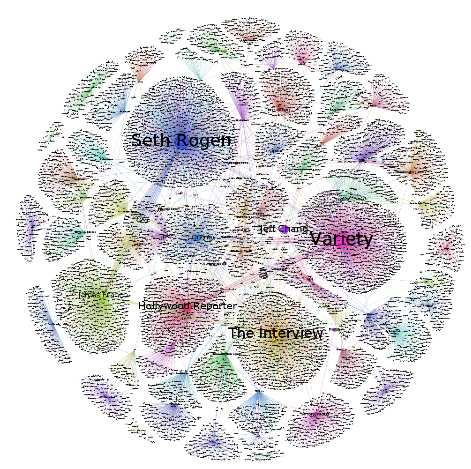
\includegraphics[width=0.6\textwidth]{interview-twitter-betweennes-centrality.png}
\caption{Highest betweenness centrality in the Fruchterman-Reingold layout for
the Twitter network of The Interview}
\end{figure}
%
\end{document}
